\documentclass[letterpaper, 12pt, notitlepage]{report}
\usepackage[plainpages=false, colorlinks, urlcolor=black, citecolor=black,
	linkcolor=blue]{hyperref}
\usepackage{graphicx}
\usepackage[utf8]{inputenc}
\usepackage{txfonts}
\usepackage{listings}
\usepackage{multirow}
\usepackage[polutonikogreek,english,spanish]{babel}
\usepackage{epsfig}
\usepackage{sty/utfsm_tesis}

%Include Table of Contents as the first entry in TOC
\usepackage{sty/xtocinc}

%\usepackage[dvips]{epsfig}
%\usepackage{psfig}

\usepackage{caption}
\usepackage{subcaption}

%% Margenes segun Normas
%% Ancho Legal 21,59cm /  8,5in
%% Alto  Legal 33,02cm / 13,0in
%\paperheight    27.81cm % alto letter
%\paperwidth     21.59cm % ancho
%\hoffset        -1.0in % Seteo a 0 el margen izquierdo
%\voffset        -1.0in % Seteo a 0 el margen superior
%\oddsidemargin  3.80cm % Margen izquierdo (pag. impar)
%% \evensidemargin 2.55cm % Margen izquierdo (pag. par) Acrobat Winkk
%\evensidemargin 2.59cm % Margen izquierdo (pag. par)
%\topmargin      1.00cm % Margen superior
%\headheight     5.00mm % Ancho encabezado
%\headsep        8.00mm % Separacion encabezado-cuerpo
%\textheight     23.5cm % Alto cuerpo
%\textwidth      15.2cm % Ancho cuerpo
%\footskip       1.30cm % Separacion piepag-cuerpo
\parindent      0em
\parskip        2ex

% Fuzz -------------------------------------------------------------------
\hfuzz2pt

% \oddsidemargin	 0cm	% Ancho Legal 21,59cm
% \evensidemargin 0.5cm	% Alto	Legal 35,56cm
% \textwidth	 16.5cm
% \topmargin	  -1.5cm
% \textheight	 22cm

\newlength{\defbaselineskip}
\setlength{\defbaselineskip}{\baselineskip}

\newcommand{\setlinespacing}[1]%
	   {\setlength{\baselineskip}{#1 \defbaselineskip}}
\newcommand{\doublespacing}{\setlength{\baselineskip}%
			   {1.3 \defbaselineskip}}
\newcommand{\singlespacing}{\setlength{\baselineskip}{\defbaselineskip}}

%Comandos de Joe
\newcommand{\jcq}[1]{``#1''}
%fin comandos de Joe

\lstloadlanguages{C++, sh, IDL, make}
\lstset{basicstyle=\small\sffamily, commentstyle=\slshape,
        numbers=left, numberstyle=\tiny, numbersep=10pt,
        extendedchars, frame=lines,
        floatplacement=ht, captionpos=b,
        defaultdialect=[CORBA]IDL}

\ingciv

\copyrightyear{2012} \submitdate{Jul 2012}
\convocation{July}{2009}

\title{Extracción de superficies a partir de una colección de puntos en un dominio tridimensional}
\author{Joe Cabezas}

\newcommand{\doctitle}{ACS Component Code Generation Framework}

\begin{document}

\selectlanguage{spanish}


\profguia{Dr. Claudio Lobos}
\profcorr{Sra. Elizabeth Montero}

%\input{include/cover.tex}
%\thispagestyle{empty}
%\input{include/cover2.tex}
%\thispagestyle{empty}
%\cleardoublepage
\vspace*{\fill}

\begin{center}
	\emph{Para mis padres, que dieron todo por mi, gracias, los amare siempre.}
\end{center}

\vspace{0.3cm}
\hspace{11cm}
\emph{Joe}

\vspace*{\fill}

%\bibliographystyle{alpha}
%\maketitle
%\frontmatter
%%\thispagestyle{empty}
%\vspace*{\fill}
%
%\selectlanguage{english}
%\begin{center}
%\begin{LARGE}\textbf{Abstract}\end{LARGE}
%\end{center}
\prefacesection{Abstract}
In this Paper, will describe the state of art of the surface extraction process from a set of 
points in a three dimensional domain, it will describe some existing techniques for this purpose 
by using examples, showing the problems and implications they present and how other techniques 
try to solve those problems.

%\selectlanguage{english}
%\newpage
%\theglossary
%\begin{table}[h!t]
	\begin{tabular}{lp{11cm}}
	Vértice   & Es el punto donde concurren las dos semirrectas que conforman un ángulo.\\

	Arista    & En geometría, el segmento de recta donde intersectan dos planos. Por extensión también se conoce con este
			nombre al segmento común que tienen dos caras vecinas de un poliedro.\\

	Poliedro  & Cuerpo geométrico cuyas caras son planas y encierran un volumen finito. La palabra poliedro
			viene del griego clásico \textgreek{polyedron} \emph{(polyedron)}, de la raíz \textgreek{poolys} \emph{(polys})
			\jcq{muchas} y de \textgreek{edra} \emph{(edra)} \jcq{base}, \jcq{asiento}, \jcq{cara}.\\

	Tetraedro & Es un poliedro de cuatro caras. Con este número de caras ha de ser un
			poliedro convexo, y sus caras triangulares, encontrándose tres de ellas en cada vértice. Si las
			cuatro caras del tetraedro son triángulos equiláteros, iguales entre sí, el tetraedro se denomina
			regular.\\

	Píxel     & Acrónimo del inglés \emph{picture element}, \jcq{elemento de imagen}, es la menor unidad homogénea en color
			que forma parte de una imagen digital.\\

	Vóxel     & Del inglés \emph{volumetric pixel}. Es una unidad cúbica que compone un objeto
			tridimensional. Constituye la unidad mínima procesable de un espacio tridimensional y es, por
			tanto, el equivalente del píxel en un objeto 3D.\\

	Dataset   & Es un conjunto de datos de entrada, para esta
			implementación, un \emph{dataset} representa un conjunto de imágenes.\\

	Isovalor	& Es un valor constante dentro del rango definido por la profundidad de 					color de las imágenes del \emph{dataset}.\\

	Isosuperficie	& Es aquella superficie que representa los puntos de un valor constante o \emph{isovalor} (presión, temperatura, etc.) dentro de un volumen en un espacio. En otras palabras, dado un espacio escalar $f(x,y,z)$ en una region $\mathbb{R}$, una \emph{isosuperficie} es una superficie determinada por el \emph{isovalor} $\alpha$, en la que todos sus puntos cumplen que $f(x,y,z) = \alpha$.\\

	%Acimut	& Es el ángulo de elevación por sobre el horizonte (o plano $XZ$), por lo que mirar hacia arriba, es lo mismo que inclinar la mirada con un acimut de $90$ grados, mientras que mirar hacia abajo es un acimut de $-90$ grados.\\

	\end{tabular}
\end{table}

%\cleardoublepage
%\tableofcontents
%\cleardoublepage
%\listoffigures
%\cleardoublepage
%\listoftables
%\cleardoublepage
%\lstlistoflistings
%\cleardoublepage
%
%\mainmatter
%\cleardoublepage

% Incluir Archivo con Agradecimientos
\ack{include/acknowledgements}

% Incluir Resumen
\resumenesp{include/abstractes}

% Incluir Abstract
\resumening{include/abstract}

% Incluir Abreviaciones
\abreviaciones{include/glossary}

\beforepreface
\afterpreface

%\numberwithin{equation}{chapter}

\chapter{Introduction}
\label{ch:introduction}

\section{Mallas Geométricas}
\label{sec:mallasGeometricas}
Las mallas de superficie son una herramienta fundamental en la ciencia e ingeniería, son
un conjunto de polígonos (triángulos, cuadriláteros, etc.), que conforman una superficie en un
espacio definido, en el que la intersección de dos elementos de una malla, puede ser el conjunto
vacío, un vértice, una arista o una cara en común. Las mallas tienen asociadas un conjunto de
elementos topológicos tales como: vértices, aristas, y caras poligonales.
Regularmente, las mallas geométricas se usan para describir, dependiendo su dimensión,
una región en un plano, o un volumen en un espacio. Realizar esta discretización consiste en
aproximar el dominio a simular dividiéndolo en elementos geométricos mas sencillos,
comúnmente triángulos, de tal manera que la intersección de dos elementos, sean un vértice, una
arista, o el conjunto vacío.

Existen casos triviales como la discretización de un dominio rectangular, cuya solución es
directa, dividiendo el dominio en un arreglo uniforme de triángulos, pero cuando se desea
discretizar un elemento de geometría irregular, la solución no es tan trivial, y se necesita de un
método de generación de mallas más elaborado.

Sin embargo, para muchos problemas de ingeniería, las mallas generadas por la
triangulación de Delaunay, no son suficientes para resolver un problema o su análisis numérico. En algunos casos es posible que sea necesario agregar nuevos puntos con el fin de mejorar la
calidad de la malla, a este proceso de mejoramiento, se le conoce como Refinamiento.

En tres dimensiones, en particular, las mallas geométricas son una representación de un
objeto físico, y para efectos de su visualización, los elementos internos de una malla pueden ser
omitidos, y con ello, sólo se utilizan mallas que describan la superficie del objeto.

\section{Usos de las Mallas Geométricas}
\label{sec:usosDeLasMallasGeometricas}
Las mallas geométricas tienen diferentes usos en la práctica, desde simulaciones físicas
tales como, estudio de fuerzas, interacción de objetos, simulación de fluidos, etc. También tienen
usos gráficos, como para hacer visualizaciones de cuerpos en tres dimensiones, visualización de
funciones matemáticas, e incluso usos artísticos como gráficos realistas, películas, etc.


\section{Consideraciones Físicas}
\label{sec:consideracionesFisicas}
En la realidad, vivimos inmersos en un mundo que podemos describirlo en tres
dimensiones, y con ello, cualquier partícula (objetos, personas, etc.) tienen una posición
específica dentro de un sistema de referencia continuo, es decir, que no existe una distancia
mínima para el desplazamiento.

Por ejemplo, usando un acercamiento a la definición de límites: si un objeto en un espacio
continuo se desplaza una distancia  d  positiva  ($d > 0$) , siempre existirá una partícula que
pueda desplazarse una distancia menor, sin importar lo pequeño que sea el valor de $d$.

Es esta continuidad del espacio del mundo real, lo que dificulta la tarea de representar
cualquier objeto en una simulación virtual.
En un espacio en tres dimensiones simulado computacionalmente, debido principalmente
a los límites de memoria de los sistemas actuales, no pueden simular un espacio continuo, sino
que todo elemento dentro de un espacio virtual debe estar inmerso en un espacio discreto, es
decir, que existe una cantidad mínima para el desplazamiento.

Los objetos en el mundo real están compuestos de materia, la que está compuesta por
átomos, la unión de ellos, crean objetos sólidos, con un nivel de detalle tan fino como atómico,
debido a la continuidad del espacio real.

Los objetos en un mundo virtual, no están (ni pueden aún), ser descritos por unidades
atómicas, ya que supondría una cantidad enorme y muy costosa de memoria para almacenar cada
átomo, y por ello, los objetos son representados por una cantidad discreta de triángulos que en
conjunto forman una superficie la cual describe la forma visible del objeto representado.

Debido a la carencia de continuidad del espacio virtual, es que los objetos representados
ahí, no son más que simples discretizaciones de los objetos reales, y en consecuencia, sin las
propiedades físicas que presentan los objetos reales, como la densidad, roce, etc.
Por ejemplo, en el mundo real, podemos pulir una superficie de manera que sea
perfectamente lisa y no presente roce, pero por muy lisa que parezca, debido a la continuidad,
podemos acercarnos de manera infinita a la superficie y notar que en realidad, aún tiene
imperfecciones que son mas pequeñas que lo mínimo visible por el ojo humano, y con ello,
eventualmente la superficie presenta roce de todas maneras por estas imperfecciones
microscópicas. Sin embargo, al representar esta superficie en el mundo virtual, simplemente
constaría de un plano perfecto en tres dimensiones, el cual, es perfectamente liso, y sin la
cantidad infinita de detalles que presenta la superficie en la realidad.

\section{Objetos en tres dimensiones}
\label{sec:objectosEnTresDimensiones}
Los objetos en tres dimensiones, como anteriormente se ejemplificó, son representados
principalmente por planos triangulares que en conjunto forman una superficie que describe la
forma externa y visible del objeto. El proceso completo para obtener un objeto en tres dimensiones, depende de la tecnología usada y el propósito por el cual se genera un modelo en
dos o tres dimensiones.

Uno de los primeros algoritmos de generación de mallas, fue el propuesto por el
matemático Ruso Boris Nikolaevich Delanuay\cite{Delaunay1934}. En honor a su autor, este algoritmo de
triangulación se denomina como el \jcq{Algoritmo de Triangulación de Delanuay}, el cual a partir de
una colección de puntos en un espacio, genera una malla geométrica formada por triángulos que
sean lo más equiláteros posible.

Para extraer la información de la forma de un cuerpo, existen tecnologías capaces de
extraer la superficie de éstos, tales como \emph{software} capaces de generar un modelo en tres
dimensiones a partir de un arreglo de fotografías que rodean al objeto, también existe la
tecnología de usar un arreglo de cámaras que capturan, en tiempo real, una nube de puntos
infrarrojos que son emitidos desde el aparato, y con ello, crear un modelo en tres dimensiones. En
el ámbito médico, también existe tecnología para poder extraer información del interior del
cuerpo humano, usando equipos de imagenología de resonancia magnética, la cual es una técnica
no invasiva que utiliza el fenómeno de la resonancia magnética para obtener información de la
estructura y composición del cuerpo a analizar, luego, la información obtenida es procesada a
través de un \emph{software} que genera la malla geométrica del área de interés por el científico.

\section{Objetivos}
\label{sec:objetivos}
En esta investigación, se propondrá un flujo de trabajo que permita la extracción de una superficie dada una colección de puntos en un espacio de tres dimensiones. Se hará enfasis en los primeros pasos del flujo propuesto, para ello se estudiará e implementará el algoritmo de \emph{Marching Cubes} para hacer la extracción de una malla de superficie que deberá ser refinada en los pasos posteriores del flujo propuesto.

Además, se construirá una herramienta de visualización y navegación que ayudará a la correcta elección del valor mínimo para poder extraer una superficie con un nivel de detalle controlable por el investigador.
\chapter{Estado del Arte}
\label{ch:estadoDelArte}

En el caso de las imágenes obtenidas por resonancia magnética, lo que se obtiene son un
arreglo de imágenes de distintos niveles en un mismo eje geométrico de un cuerpo. Luego, para
generar una malla geométrica del cuerpo existen diversas técnicas, muchas de ellas basadas en
\jcq{voxels} como por ejemplo, Marching Cubes\cite{Lorensen87marchingcubes}, Marching Tetrahedrons\cite{Shirley90apolygonal} y Marching Diamonds.
En esta investigación se dará especial énfasis en el algoritmo de Marching Cubes, se
explicará su funcionamiento, resultados y problemas que actualmente presenta.
Para entender mejor cómo funciona Marching Cubes, es de utilidad primero ver el caso
reducido a dos dimensiones, el que puede ser llamado como \jcq{Marching Squares}.

\section{Marching Squares}
\label{sec:marchingSquares}

En dos dimensiones, para obtener el contorno de una figura, se puede usar este algoritmo
que se basa en crear divisiones cuadradas uniformes del espacio, y en cada una de ellas dibujar un
patrón específico del caso que encierra esa división, finalmente todas las divisiones tienen
dibujadas un patrón específico o un espacio vacío, obteniendo así el contorno de la imagen
tratada. El siguiente caso, ejemplifica el proceso completo.

Se supone la imagen de la figura \ref{f:estadoDelArte:original} para tratar obtener su contorno.

\begin{figure}
	\centering
		\fbox{
			
\includegraphics[width=0.7\textwidth]{images/marchingsquare/original.jpg}
		}
	\caption{Figura original de estudio, a la que se desea extraer su contorno}
	\label{f:estadoDelArte:original}
\end{figure}

Luego se divide el espacio en un arreglo uniforme de cuadriláteros, en este caso una
matriz de 7x8 celdas como muestra la figura \ref{f:estadoDelArte:division}

Para poder obtener el patrón a dibujar en cada celda, se hace un proceso de
reconocimiento. En un principio es necesario etiquetar cada vértice de cada celda dependiendo si
están dentro o fuera de la región de interés. Esto puede ser calculado de distintas formas que
dependen intrínsecamente del problema, para este caso, basta con detectar si el vértice está sobre
un pixel blanco o no, en otros casos, puede depender de que si el valor del pixel en escala de
grises supera (o es inferior) a un valor fijo determinado por el científico.

\begin{figure}
	\centering
		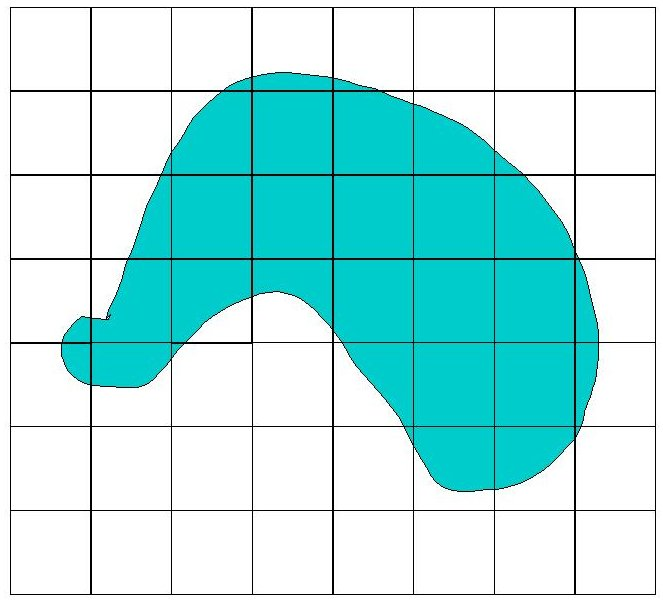
\includegraphics[width=0.7\textwidth]{images/marchingsquare/division.jpg}
	\caption{Figura original dividida en un arreglo uniforme de celdas}
	\label{f:estadoDelArte:division}
\end{figure}

A continuación, se muestra como quedan etiquetados los vértices, dependiendo si están
dentro de la figura (en rojo), o si están fuera de la figura (en azul), como muestra la figura \ref{f:estadoDelArte:labeledobj}

\begin{figure}
	\centering
		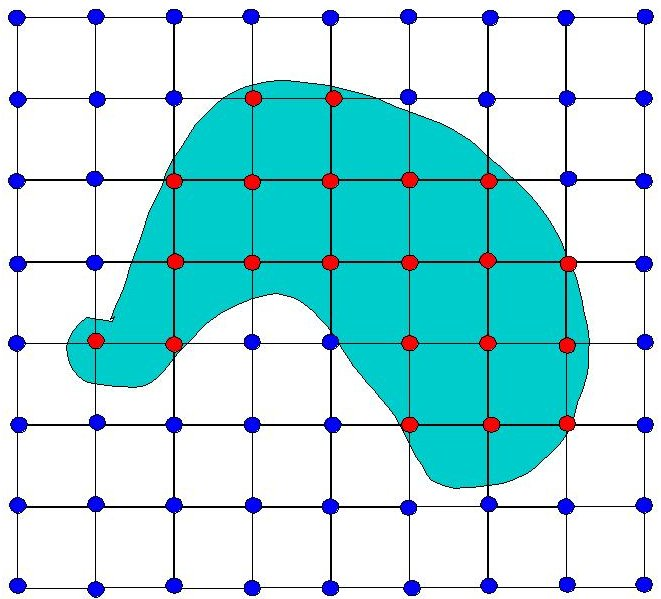
\includegraphics[width=0.7\textwidth]{images/marchingsquare/labeledobj.jpg}
	\caption{Etiquetado de vértices según su condición relativa a la figura}
	\label{f:estadoDelArte:labeledobj}
\end{figure}

Si ahora se analiza celda a celda, se ve que existen dieciséis combinaciones distintas de
vértices etiquetados como dentro o fuera de la región en una misma celda, como muestra la figura
\ref{f:estadoDelArte:cases}

\begin{figure}
\centering
	\fbox{
		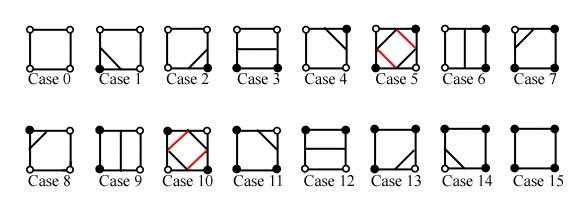
\includegraphics[width=\textwidth]{images/marchingsquare/cases.jpg}
	}
\caption{Los dieciséis casos posibles en Marching Squares}
\label{f:estadoDelArte:cases}
\end{figure}

Además se entiende que si uno de los lados de una celda (una arista) esta formada por un
vértice marcado como dentro y otro fuera, significa que por esa arista corta el borde de la figura,
y por lo tanto, esa arista la dejamos marcada como una arista de contorno detectada, que en este
ejemplo se marca de color morado, como muestra la figura \ref{f:estadoDelArte:purpledobj}

\begin{figure}
\centering
	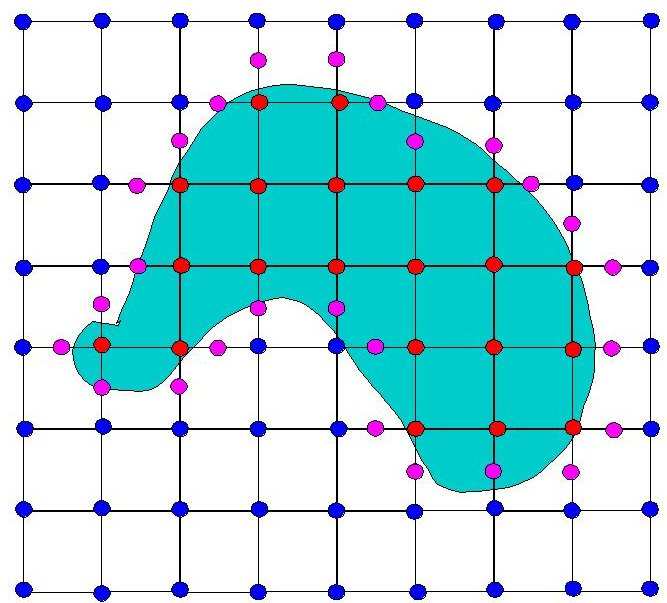
\includegraphics[width=0.7\textwidth]{images/marchingsquare/purpledobj.jpg}
\caption{Aristas marcadas por las cuales cortará el contorno calculado}
\label{f:estadoDelArte:purpledobj}
\end{figure}

Luego, por cada celda, se unen los puntos morados formados en el paso anterior, creando
así uno de los dieciséis patrones posibles, lo cual se puede entender como una de las dieciséis
formas en que un cuadrilátero puede ser atravesado por una linea, formando así el contorno
buscado, como muestra la figura \ref{f:estadoDelArte:connectedobj}

\begin{figure}
\centering
	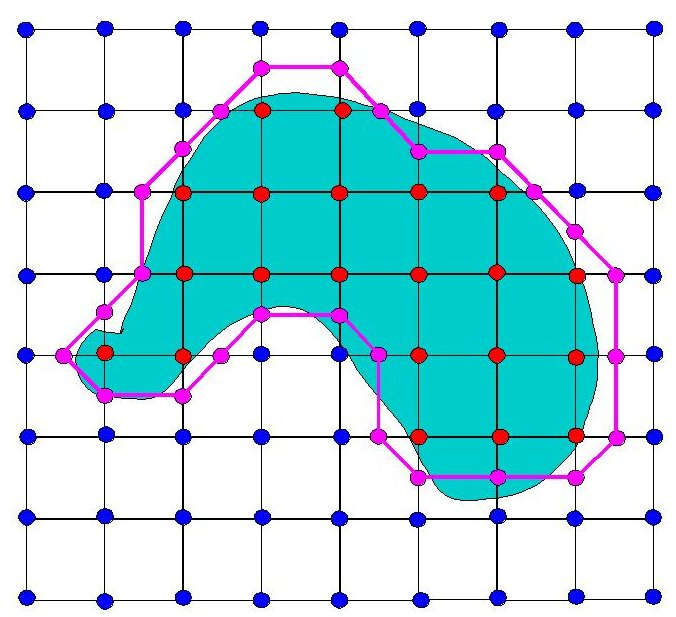
\includegraphics[width=0.7\textwidth]{images/marchingsquare/connectedobj.jpg}
\caption{Contorno calculado usando las aristas marcadas en el paso anterior}
\label{f:estadoDelArte:connectedobj}
\end{figure}

Posteriormente, dependiendo de los requerimientos de la investigación, se puede mejorar
la aproximación haciendo una interpolación lineal de los valores de los vértices para calcular en
que punto aproximadamente la figura (a la que se quiere extraer su contorno), corta con la arista,
un ejemplo del resultado de esta aproximación se muestra en la figura \ref{f:estadoDelArte:2Dintersected}

\begin{figure}
\centering
	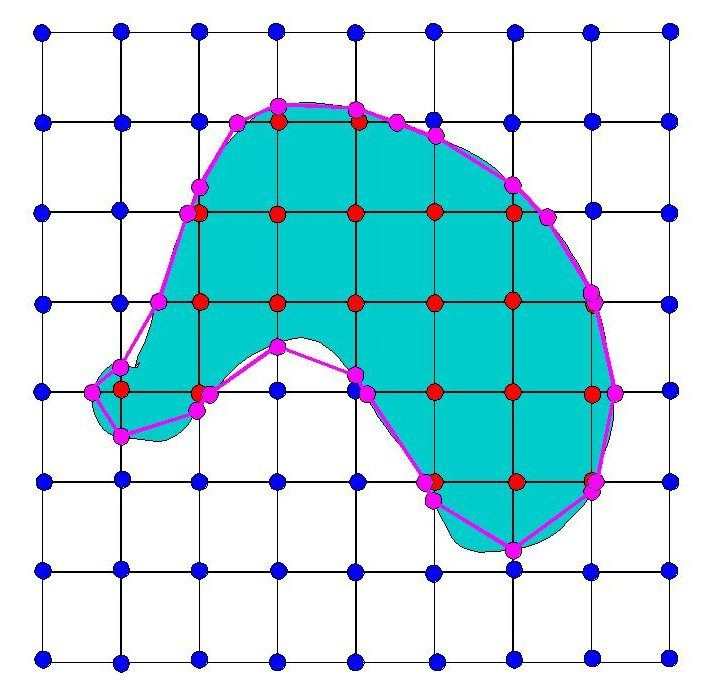
\includegraphics[width=0.7\textwidth]{images/marchingsquare/2Dintersected.jpg}
\caption{Mejorando la calidad del contorno usando interpolación lineal}
\label{f:estadoDelArte:2Dintersected}
\end{figure}

\subsection{Consecuencias}
\label{subsec:marchingSquares:consecuencias}

Evidentemente, existen ciertas falencias, por ejemplo, el contorno obtenido no simula
adecuadamente el objeto estudiado, debido a errores causados por la fragmentación de las
divisiones iniciales, una solución directa para mejorar esto es aumentar las divisiones, es decir,
hacer que todas las celdas sean mas pequeñas, y así hacer una mejor aproximación del contorno
del objeto en estudio. De la misma manera, existen otras técnicas, tales como hacer particiones
con celdas de tamaño variable en las particiones, o subdividir aquellas celdas que hayan sido
detectadas como de frontera y así obtener un mejor desempeño en el algoritmo.

Otro problema es que algunos casos presentan ambigüedad, es decir, no es trivial calcular
a cual caso pertenece una cierta configuración, por ejemplo, tomando el quinto y décimo caso
descritos anteriormente, se supone el ejemplo descrito por la figura \ref{f:estadoDelArte:marchingSAmbEx}

\begin{figure}[hbp]
\centering
	\fbox{
		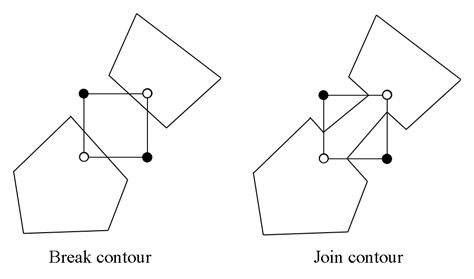
\includegraphics[width=0.7\textwidth]{images/marchingsquare/marchingSAmbEx.jpg}
	}
\caption{Casos con ambigüedad}
\label{f:estadoDelArte:marchingSAmbEx}
\end{figure}

Este cuadrado, tiene dos vértices diagonalmente opuestos marcados. Sin conocer como es
la figura ni cómo son las divisiones vecinas, no se puede saber con exactitud si se trata del quinto
o el décimo caso, por lo que el algoritmo puede erróneamente separar el contorno, formando así
dos figuras separadas, o las une, de manera que sólo exista una figura con un contorno
compartido.

\section{Marching Cubes}
\label{sec:marchingCubes}

\subsection{Idea}
\label{subsec:marchingCubes:idea}

Marching Cubes es un algoritmo de extracción de una superficie poligonal de un cuerpo
en un espacio escalar en tres dimensiones \cite{Lorensen87marchingcubes}. Existen muchas aplicaciones para este tipo de técnicas,
dos de las más comunes son:

\begin{itemize}
	\item Reconstrucción de una superficie a partir de un set de imágenes médicas, como
	por ejemplo los obtenidos en imágenes de resonancia magnética, los que pueden formar
	un volumen en tres dimensiones.

	\item Crear un contorno tridimensional de un campo escalar matemático, en este caso,
	el valor de una cierta función es conocido en todo el espacio, pero es representada como
	vértices de una malla tridimensional.
\end{itemize}

Adopta la misma idea que hay detrás de Marching Squares, pero llevando los conceptos a
tres dimensiones, en este caso, el dominio es un espacio tridimensional, en el cual existe un
cuerpo al que se desea extraer su superficie. Luego, el espacio es dividido en regiones uniformes
(cubos), por los cuales la superficie del objeto corta las aristas de estos cubos.

\subsection{Consideraciones Geométricas}
\label{subsec:marchingCubes:consideracionesGeometricas}

Un cubo tiene seis caras, ocho vértices y doce aristas, las cuales, para efectos de esta
investigación serán numeradas como se muestra en la figura \ref{f:estadoDelArte:convention}

%TODO: al parecer quiza sea necesario usar una convencion equitativa, pero rotada
%para que considere los dataset como son interpretados, es decir, con Y positivo
%apuntando hacia abajo, y Z en direccion a donde se van poniendo las imagenes
%		3	2
%	0	1
%		7	6
%	4	5
\begin{figure}[hbp]
\centering
	\fbox{
		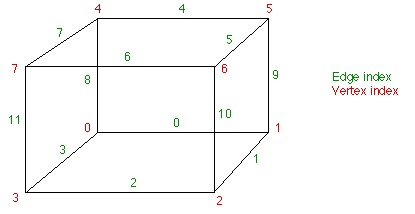
\includegraphics[width=0.9\textwidth]{images/marchingcubes/convention.jpg}
	}
\caption{Convención de enumeración de vértices y aristas}
\label{f:estadoDelArte:convention}
\end{figure}

De la misma manera que el caso de dos dimensiones, debido a que cada uno de los ocho
vértices puede tener dos estados: vértice marcado como interno o externo (dentro o fuera de la
superficie del cuerpo), se tienen 256 combinaciones posibles, es decir, una superficie puede
atravesar a un cubo de 256 maneras posibles. Sin embargo, al igual que en su homólogo en dos
dimensiones, que tiene dieciséis formas posibles, estas pueden ser reducidas a un número inferior
de patrones, ya que entre ellos existen diferencias solamente de rotación y reflexión.

En el caso de tres dimensiones, los 256 patrones pueden ser reducidos de la misma
manera. Dos de esos casos son triviales, ya que tienen todos sus vértices marcados como internos
o externos, por lo tanto, ambos casos no contribuyen a la superficie que se quiere extraer.

Si se consideran las simetrías, hay solamente catorce posibles configuraciones únicas en
los restantes 254 casos. Por ejemplo, aquellos casos que solamente tienen un vértice marcado
como interno, sólo representan un triángulo que atraviesa las aristas que convergen a ése vértice y
existen ocho casos como éste, uno por cada vértice del cubo.

Finalmente las quince familias de posibles casos son los que se describen en la figura \ref{f:estadoDelArte:Shu95adaptivemarching_1}

\begin{figure}[hbp]
\centering
	\fbox{
		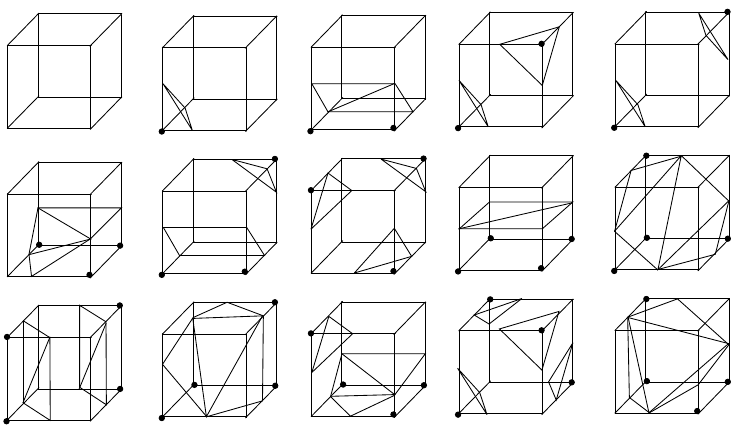
\includegraphics[width=0.9\textwidth]{images/marchingcubes/Shu95adaptivemarching_1.png}
	}
\caption{Los quince casos de Marching Cubes \cite{Shu95adaptivemarching}}
\label{f:estadoDelArte:Shu95adaptivemarching_1}
\end{figure}

\subsection{Procedimiento}
\label{subsec:marchingCubes:procedimiento}

El procedimiento es similar al explicado a Marching Squares, en primer lugar se divide el
espacio en un arreglo uniforme de regiones cúbicas, luego, se evalúa cada vértice para etiquetarlo como un vértice interno o externo, luego, calcular a cuál de los 15 casos pertenece cada división y generar los triángulos, para finalmente extraer así la superficie.
En resumen, el procedimiento reducido a un solo cubo, ocurre según lo siguiente:

En un comienzo se tiene un cubo, como el descrito en la figura \ref{f:estadoDelArte:cube_01}

\begin{figure}[hbp]
\centering
	\fbox{
		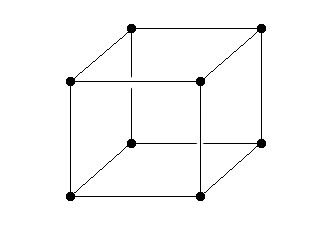
\includegraphics[width=0.4\textwidth]{images/marchingcubes/cube_01.png}
	}
\caption{Un cubo con sus vértices marcados}
\label{f:estadoDelArte:cube_01}
\end{figure}

Suponiendo que este cubo tiene solamente un vértice que quedó dentro del cuerpo, éste
vértice queda marcado como un vértice interno (en rojo), los siete restantes quedan marcados
como vértices externos (en negro), descrito por le figura \ref{f:estadoDelArte:cube_02}

\begin{figure}[hbp]
\centering
	\fbox{
		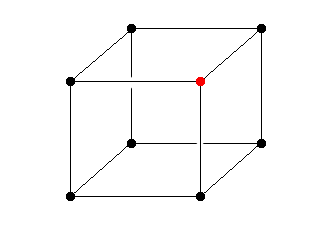
\includegraphics[width=0.4\textwidth]{images/marchingcubes/cube_02.png}
	}
\caption{Un cubo con uno de sus vértices marcado como interno}
\label{f:estadoDelArte:cube_02}
\end{figure}

Luego se crea un triángulo cuyos vértices se apoyan en los puntos medios de las aristas
que comparten el vértice marcado como interno, de esta manera, se tiene un cubo que es
atravesado por una superficie que precisamente deja un solo vértice dentro (o fuera, dependiendo
de la reflexión del caso), resultando un triángulo como el de la figura \ref{f:estadoDelArte:cube_03}

\begin{figure}[ht]
\centering
	\fbox{
		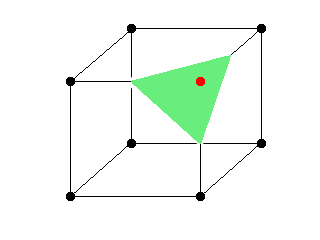
\includegraphics[width=0.4\textwidth]{images/marchingcubes/cube_03.png}
	}
\caption{Un triángulo atraviesa el cubo separando el vértice marcado de los demás}
\label{f:estadoDelArte:cube_03}
\end{figure}

\subsection{Consecuencias}
\label{subsec:marchingCubes:consecuencias}

Nuevamente, al igual que su versión en dos dimensiones, presenta las mismas falencias.
Por ejemplo, sin ninguna interpolación y dependiendo de la resolución de la división, la
superficie extraída puede presentar un efecto de escalonamiento (\jcq{aliasing}) como se
muestra en la figura \ref{f:estadoDelArte;superficies_resultantes_variando_divisiones}

\begin{figure}

	\begin{subfigure}{0.45\textwidth}
		\centering
		\includegraphics[width=\textwidth]{images/marchingcubes/mc_blobs.png}
		\caption{La forma original}
		\label{f:estadoDelArte:mc_blobs}
	\end{subfigure}
	~
	\begin{subfigure}{0.45\textwidth}
		\centering
		\includegraphics[width=\textwidth]{images/marchingcubes/mc_blobs_12.png}
		\caption{Marching Cubes con 12 divisiones}
		\label{f:estadoDelArte:mc_blobs_12}
	\end{subfigure}

	\begin{subfigure}{0.45\textwidth}
		\centering
		\includegraphics[width=\textwidth]{images/marchingcubes/mc_blobs_20.png}
		\caption{Marching Cubes con 20 divisiones}
		\label{f:estadoDelArte:mc_blobs_20}
	\end{subfigure}
	~
	\begin{subfigure}{0.45\textwidth}
		\centering
		\includegraphics[width=\textwidth]{images/marchingcubes/mc_blobs_50.png}
		\caption{Marching Cubes con 50 divisiones}
		\label{f:estadoDelArte:mc_blobs_50}
	\end{subfigure}

	\caption{Superficies resultantes variando la cantidad de divisiones}
	\label{f:estadoDelArte;superficies_resultantes_variando_divisiones}
\end{figure}

Se puede apreciar que al aumentar la resolución, la calidad aumenta, pero
computacionalmente requiere mas cómputo y memoria ya que aumenta la cantidad de caras que
describen la superficie extraída como se ve en la figura \ref{f:estadoDelArte:polygonise3}

\begin{figure}[!ht]
\centering
	\fbox{
		\includegraphics[width=0.9\textwidth]{images/marchingcubes/polygonise3.png}
	}
\caption{Ejemplificación de cómo varían los resultados al modificar la resolución}
\label{f:estadoDelArte:polygonise3}
\end{figure}

El principal problema de \emph{Marching Cubes} es que existe la posibilidad de que aparezcan agujeros como el resultado de la discrepancia en la conexión de los vértices en una cara en común de dos cubos adyacentes \cite{Chernyaev95marchingcubes}

Como se muestra en la figura \ref{f:estadoDelArte:Bloomenthal88polygonizationof_1}, la poligonización puede producir casos ambigüos cuando en una cara de un cubo quedan marcados dos vértices opuestos (que no comparten ninguna arista), ya que no es posible decidir si la superficie corta en multiples partes el cubo o un cilindro atraviesa las dos esquinas opuestas.

\begin{figure}[t]
\centering
	\fbox{
		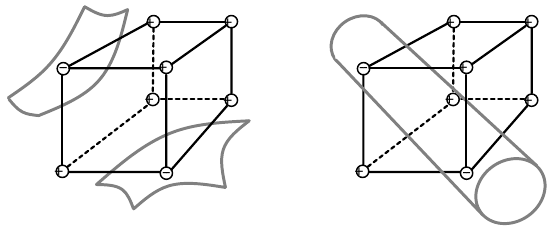
\includegraphics[width=0.7\textwidth]{images/marchingcubes/Bloomenthal88polygonizationof_1.png}
	}
\caption{Casos en los que se generan errores topológicos}
\label{f:estadoDelArte:Bloomenthal88polygonizationof_1}
\end{figure}

Es por esto que si se forma una configuración en la que dos cubos comparten una cara las cuales tienen solo dos vértices opuestos marcados, pueden generar agujeros en el modelo final en tres dimensiones, como se grafica en la figura \ref{f:estadoDelArte:Chernyaev95marchingcubes_1}

\begin{figure}[!htb]
\centering
	\fbox{
		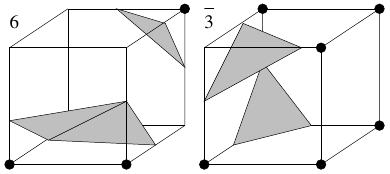
\includegraphics[width=0.5\textwidth]{images/marchingcubes/Chernyaev95marchingcubes_1.png}
	}
\caption{Un agujero causado por una cara con ambigüedad compartida por dos cubos \cite{Chernyaev95marchingcubes}}
\label{f:estadoDelArte:Chernyaev95marchingcubes_1}
\end{figure}

Otro problema puede incluso aparecer cuando no hay discrepancias visibles, \emph{Marching Cubes} puede producir \emph{isosuperficies} con una topología diferente a la generada por otros métodos en el mismo caso \cite{Chernyaev95marchingcubes}. La figura \ref{f:estadoDelArte:Chernyaev95marchingcubes_2} muestra las \emph{isosuperficies} generadas para el mismo cubo usando dos metodos distintos, el primer método se realizó usando \emph{Marching Cubes} y el otro usando \emph{Dividing Cubes Method} \cite{Cline88twoalgorithms}, el cual subdivide el cubo en regiones cúbicas mas pequeñas. La superficie generada por \emph{Marching Cubes} consiste en dos triángulos separados, mientras que la superficie generada por \emph{Dividing Cubes Method} parece mas un \jcq{tubo}

\begin{figure}[!htb]
\centering
	\fbox{
		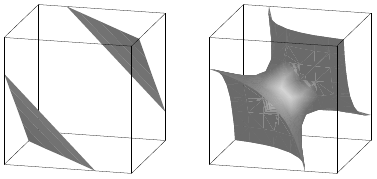
\includegraphics[width=0.5\textwidth]{images/marchingcubes/Chernyaev95marchingcubes_2.png}
	}
\caption{\emph{isosuperficies} generadas por dos métodos diferentes \cite{Chernyaev95marchingcubes}}
\label{f:estadoDelArte:Chernyaev95marchingcubes_2}
\end{figure}

Resolviendo las ambigüedades, se pueden evitar los agujeros, de todas maneras, esto no garantiza una topología correcta \cite{Lewiner03efficientimplementation}, tambien es necesario resolver las ambigüedades internas, causadas por aquellos casos que tienen vértices marcados y diagonalmente opuestos. Por ejemplo, para un mismo caso, pueden existir dos posibles poligonizaciones que resuelven el caso y son topológicamente distintas como se muestra en la figura \ref{f:estadoDelArte:Lewiner03efficientimplementation_2}

\begin{figure}[!htb]
\centering
	\fbox{
		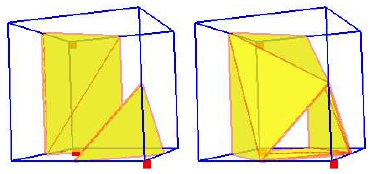
\includegraphics[width=0.5\textwidth]{images/marchingcubes/Lewiner03efficientimplementation_2.png}
	}
\caption{Dos posibles poligonizaciones para el mismo caso, ambas resuelven los dos posibles casos de ambigüedad \cite{Lewiner03efficientimplementation}}
\label{f:estadoDelArte:Lewiner03efficientimplementation_2}
\end{figure}

Estos problemas pueden ser eliminados si se usa una particion del espacio usando \emph{simplexs}\cite{Bloomenthal88polygonizationof}.
Un \emph{simplex} es la descomposición lineal más simple de un n-espacio. Para tres dimensiones, es el tetraedro. Cualquier par de vértices de un tetraedro esta unido por una arista en común, y por lo tanto, cualquier vértice marcado puede ser separado del resto usando solamente un plano.

% Para poder evitar estos errores, se introducen seis nuevas familias de casos, que están descritas en
% la figura \ref{f:estadoDelArte:MCAmb}

% \begin{figure}[htb]
% \centering
% 	\fbox{
% 		\includegraphics[width=0.8\textwidth]{images/marchingcubes/MCAmb.png}
% 	}
% \caption{Nuevos patrones que solucionan los errores topológicos}
% \label{f:estadoDelArte:MCAmb}
% \end{figure}

% En el ejemplo anterior, en vez de usar el patrón etiquetado como 6e, debería usarse el 6c
% de la figura anterior, solucionando así el potencial error topológico.
% Otra posible solución, es usar pirámides o tetraedros (Marching Tetrahedrons \cite{Shirley90apolygonal}), los cuales
% son más sencillas de utilizar ya que sólo existen 16 posibles combinaciones totales (al igual que
% Marching Squares, ya que en ambos casos, los elementos tienen cuatro vértices), los cuales
% pueden ser reducidos a sólo cuatro. La poligonización tetraédrica se muestra en la figura \ref{f:estadoDelArte:image_004}

\begin{figure}[htb]
\centering
	\fbox{
		\includegraphics[width=0.9\textwidth]{images/marchingtetrahedrons/image_004.png}
	}
\caption{Poligonización tetraédrica}
\label{f:estadoDelArte:image_004}
\end{figure}

De hecho, en el caso de Marching Cubes, cada cubo puede al final, descomponerse en
cinco pirámides o tetraedros como se muestra en la figura \ref{f:estadoDelArte:image_006}

\begin{figure}[htb]
\centering
	\fbox{
		\includegraphics[width=0.7\textwidth]{images/marchingtetrahedrons/image_006.png}
	}
\caption{Descomposición tetraédrica de un cubo}
\label{f:estadoDelArte:image_006}
\end{figure}

\chapter{Propuesta}
\label{ch:Propuesta}
\chapter{Implementación}
\label{ch:implementacion}

\section{Estructura}
\label{ch:implementacion:sec:estructura}

Para realizar la implementacion del algoritmo se debe primero proponer una convención para enumerar los vertices y aristas de un cubo, para esta implementacion se usara la convencion señalada anteriormente en la figura \ref{f:estadoDelArte:convention}, luego de definida la enumeración de cada vértice y arista, es necesario poder representar cada uno de los 256 casos con un identificador único denominado \emph{cubeIndex}, luego hay que determinar que aristas son cortadas por la superficie que atraviesa cada caso en particular, para ello se necesita de una tabla que asocie un \emph{cubeIndex} con las aristas que seran atravesadas, esta tabla se denomina \emph{edgeTable}, una vez que se conocen aquellas aristas que son atravesadas, el siguiente paso es crear una malla de triángulos que formen esta superficie, la tabla \emph{triTable} asocia cada caso con una lista de triángulos ordenados, que generan la superficie buscada. Todas estas estructuras de datos serán explicadas a continuación.

\section{Estructuras de datos}
\label{ch:implementacion:sec:estructurasDeDatos}

\subsection{CubeIndex}
\label{ch:implementacion:sec:CubeIndex}

Como se menciono en \ref{subsec:marchingCubes:consideracionesGeometricas}, existen 256 formas posibles de atravesar un cubo con una superficie continua, que es lo mismo decir, existen 256 combinaciones posibles dados 8 vertices que pueden estar en 2 estados distintos (indicando que estan dentro de una superficie cerrada o fuera de ésta)

Para poder identificar cada uno de estos 256 casos, se enumeran del 1 al 256 usando un arreglo de 8 bits, basandose en el estado de cada vertice usando la convención, por ejemplo, un cubo que tiene todos sus vértices marcados como fuera de la superficie (externos), tiene todos sus bits en cero, por lo tanto, el índice, desde ahora \emph{cubeIndex}, de este cubo es \hbox{$0_{10} = 0000 \; 0000_{2}$} (cero), de la misma manera, usando la convención, si un cubo sólo tiene el tercer vertice (vertice 2), dentro de la superficie, entonces, tiene su tercer bit en 1, y el resto en cero, luego el \emph{cubeIndex} del cubo es $4_{10} = 0000 \; 0100_{2}$, si un cubo es atravesado por la mitad, dejando a la mitad de abajo dentro de la superficie, tiene los vértices 4, 5, 6 y 7 marcados como internos, por lo que los bits 4, 5, 6 y 7 (los ultimos 4), valen 1, por lo tanto, el \emph{cubeIndex} es $240_{10} = 1111 \; 0000_{2}$.

En general, el \emph{cubeIndex} se determina como se muestra en la figura \ref{f:ch:implementacion:sec:CubeIndex:cubeindex:cubeindex}.

\begin{figure}[hbt]
	\makebox[\textwidth]{\framebox[0.3\textwidth]{\rule{0pt}{0.2\textwidth}}}
	\caption{Five by Five in Centimetres.}
	\label{f:ch:implementacion:sec:CubeIndex:cubeindex:cubeindex}
\end{figure}

\subsection{edgeTable}
\label{ch:implementacion:sec:edgeTable}

Luego de establecer como identificar un cubo, es necesario poder conocer que aristas serian intersectadas por la superficie, para poder determinar un punto sobre estas aristas por las cuales se sostendrá un triángulo. Por ejemplo, si el vértice $0$, es el unico vértice que queda dentro de la superficie, usando la convención, se puede asumir las aristas $0$, $3$ y $8$ seran aquellas las cuales la superficie intersectara a cubo.

Es por esto que se necesita una forma de relacionar un \emph{cubeIndex} con las aristas que serán atravesadas por la superficie.

Usando la misma estrategia que con el \emph{cubeindex} existen 4096 $(2^{12})$ combinaciones posibles de tomar 12 aristas que pueden intersectar a la superficie o no, por esto, cada caso, será identificado con un numero de 12 bits, en el cual, cada bit representa a una arista, usando la convención como se muestra en la figura \ref{f:ch:implementacion:sec:CubeIndex:edgeTable:edge_convention}.

\begin{figure}[hbt]
	\makebox[\textwidth]{\framebox[0.4\textwidth]{\rule{0pt}{0.3\textwidth}}}
	\caption{Convención para enumerar las 4096 combinaciones posibles de aristas}
	\label{f:ch:implementacion:sec:CubeIndex:edgeTable:edge_convention}
\end{figure}

La \emph{edgeTable} es un \emph{array} (arreglo) diseñado para asociar un \emph{cubeindex} con quellas aristas que son intersectadas. este \emph{array} consta de 256 numeros (uno por cada caso o cada \emph{cubeindex}) de 12 bits, un bit para cada una de las 12 aristas del cubo en cuestión por las cuales pasa la superficie.

Para entender mejor, se supone el ejemplo de la figura \ref{f:ch:implementacion:sec:CubeIndex:edgeTable:example}.

\begin{figure}[hbt]
	\makebox[\textwidth]{\framebox[0.3\textwidth]{\rule{0pt}{0.2\textwidth}}}
	\caption{Five by Five in Centimetres.}
	\label{f:ch:implementacion:sec:CubeIndex:edgeTable:example}
\end{figure}

En este ejemplo, sólamente el vértice $0$, ha sido marcado como interno, luego, el \emph{cubeIndex} es $1_{10} = 0000 \; 0001_{2}$, dado esto, las aristas $0$, $3$ y $8$ serán eventualmente atravesadas por la superficie, por lo tanto:

\begin{quote}
	edgeTable[1] = 0x109
\end{quote}

Lo cual tiene un valor equivalente a: $109_{16} = 265_{10} = 0001 \; 0000 \; 1001_{2}$, lo que indica, viendo la notacion binaria, que las aristas $0$, $3$ y $8$ son las que serán atravesadas.

Otro ejemplo, se supone el caso de la figura \ref{f:ch:implementacion:sec:CubeIndex:edgeTable:example}

\begin{figure}[hbt]
	\makebox[\textwidth]{\framebox[0.3\textwidth]{\rule{0pt}{0.2\textwidth}}}
	\caption{Five by Five in Centimetres.}
	\label{f:ch:implementacion:sec:CubeIndex:edgeTable:example}
\end{figure}

En este caso, los vértices $5$ y $6$ han sido marcados como internos, luego, el \emph{cubeIndex} debe ser: $96_{10} = 0110 \; 0000_{2}$, por lo tanto la superficie deberia atravesar las aristas $4$, $9$, $6$ y $10$, para que asi, una superficie deje a estos vértices separados del resto.

Para saber que aristas finalmente son atravesadas, se debe consultar a la tabla \emph{edgeTable}, usando como índice, el \emph{cubeIndex} calculado anteriormente.

\begin{quote}
	edgeTable[96] = 0x650
\end{quote}

El valor entregado por la \emph{edgeTable} para el \emph{cubeIndex} $96$, es $0x650$ (hexadecimal), lo que es equivalente a:

\begin{quote}
	$650_{16} = 1616_{10} = 0110 \; 0101 \; 0000_{2}$
\end{quote}

Según la notación binaria, se puede ver que el valor entregado por la tabla \emph{edgeTable}, indica que los vertices $4$, $6$, $9$ y $10$ son aquellos que son atravesados por la superficie, de forma que los vertices $5$ y $6$ queden separados del resto.

\subsection{triTable}
\label{ch:implementacion:sec:triTable}

Una vez que se conocen aquellas aristas que seran atravesadas, es momento de crear la superficie interna que atraviese estas aristas y separe los vertices marcados de los demás. Para ello, es necesario poder generar aquellos triángulos que formen esta superficie.

la tabla \emph{triTable} es una tabla de 256 \emph{arrays} (arreglos) de 16 numeros cada uno, hay un arreglo por cada uno de los 256 casos descritos en \ref{ch:implementacion:sec:CubeIndex}, en cada caso, es necesario generar una serie de triángulos que describirán la superficie, y de todos los casos, como máximo se necesitan 5 triángulos para los casos mas complejos.

Analizando un caso simple, un cubo que solamente tiene un vértice marcado, por lo tanto se necesita tan sólo un triángulo que se sostenga de las aristas que convergen en ese vertice, para asi crear una superficie que atraviese el cubo dejando a ese vértice separado del resto de los vértices del cubo, es por esto, que el segundo elemento (\emph{cubeIndex} = 1) de la tabla \emph{triTable} tiene un valor:

\begin{quote}
	$triTable[1] = \{0, 8, 3, -1, -1, -1, -1, -1, -1, -1, -1, -1, -1, -1, -1, -1\}$
\end{quote}

Esto indica que el primer triángulo, es aquel que se sostiene (o corta) de las aristas: $0$, $8$ y $3$.

El resto de los $13$ números que quedan tienen un valor de $-1$, lo cual permite a cualquier implementacion del algoritmo, iterar en los numeros como tripletas, y detenerse cuando el primer número tenga un valor de $-1$.

De esta manera, cuando un cubo no tiene ninguno de sus vértices marcados (\emph{cubeIndex} = 0), o tiene todos sus vértices marcados (\emph{cubeIndex} = 255), los valores de la triTable para ambos casos son:

\begin{quote}
	$triTable[0]	= \{-1, -1, -1, -1, -1, -1, -1, -1, -1, -1, -1, -1, -1, -1, -1, -1\}$\\
	$triTable[255]	= \{-1, -1, -1, -1, -1, -1, -1, -1, -1, -1, -1, -1, -1, -1, -1, -1\}$
\end{quote}

Esto indica que para ambos casos, no se crea ningún trianglo, ya que cuando no tiene ningún vértice marcado indica que esta completamente fuera de la superficie, o en el otro caso, el cubo está contenido completamente dentro de la superficie, y ambos casos deben ser reemplazados por un cubo con cero triangulos.

\section{Datos de entrada}
\label{ch:implementacion:sec:datosDeEntrada}

\subsection{Requerimientos}
\label{ch:implementacion:sec:datosDeEntrada:subsec:requerimientos}

Para poder utilizar el algoritmo de \emph{MarchingCubes}, se necesita que cada punto de un espacio tridimensional tenga asociado un valor dentro de un rango definido de manera que cada punto pueda describirse como un vector de cuatro dimensiones compuestas por sus coordenadas y un valor escalar, como muestra la ecuacion \ref{ch:implementacion:sec:datosDeEntrada:vector}.

\begin{equation}
\label{ch:implementacion:sec:datosDeEntrada:vector}
	(x,y,z,v)
\end{equation}

Por ejemplo, en una habitación se tiene un foco de luz en el centro emitiendo luz en todas direcciones, con esto, cada punto de la habitación percibe distintas instensidades de luz que depende de la distancia al foco, mientras mas cerca del foco, mayor intensidad, mientras mas alejado del foco, menor intensidad. Si de alguna manera pudiesen marcase todos aquellos puntos que tengan una intensidad especifica se tendria una esfera formada por puntos equidistantes al foco, ya que todo ellos comparten la misma intensidad, por lo que se dice que esa es la superficie que encierra a todos los puntos con una cierta intensidad o mayor.

Ciertamente, el algoritmo tambien sirve para visualizar graficos en tres dimensiones, usando el mismo principio, cada punto del espacio tiene un valor asociado el cual es calculado por la ecuacion, para poder dibujar la susperficie se puede transformar la ecuacion en una inecuacion y luego marcar todos aquellos puntos que sean menores que el valor entregado por la ecuacion, por ejemplo se tiene en la ecuación \ref{ch:implementacion:sec:datosDeEntrada:ec1}:

\begin{equation}
\label{ch:implementacion:sec:datosDeEntrada:ec1}
	x^{2} + y^{2} = 1
\end{equation}

Para poder graficar esta ecuacion usando \emph{MarchingCubes} se debe transformar la ecuación en una inecuación como se muestra en la ecuacion \ref{ch:implementacion:sec:datosDeEntrada:ec2}:

\begin{equation}
\label{ch:implementacion:sec:datosDeEntrada:ec2}
	x^{2} + y^{2} <= 1
\end{equation}

Dependiendo de la resolución escogida, es posible que algunos cubos tengan algunos de sus vértices con coordenadas $(x,y)$ que satisfacen a la inecuación, por lo tanto quedan marcados como vértices internos, luego el proceso es ir iterando en todos esos cubos y reemplazando los cubos por los triangulos que correspondan a los quince casos mostrados en la figura \ref{f:estadoDelArte:MarchingCubes}.

\subsection{Datos como cortes de nivel}
\label{ch:implementacion:sec:datosDeEntrada:subsec:datoscomocurvasdenivel}

Otra forma de entregar datos de entrada es teniendo cortes de nivel de un cuerpo tridimensional, un ejemplo de esto son las imágenes obtenidas de los exámenes de resonancia magnética. Cada imagen representa un corte transversal del cuerpo estudiado, como el que se muestra en la figura \ref{f:ch:implementacion:sec:datosdeentrada:img:ejemplodernm}:

\begin{figure}[hbt]
	\makebox[\textwidth]{\framebox[0.5\textwidth]{\rule{0pt}{0.5\textwidth}}}
	\caption{Imágenes una resonancia magnética de abdomen completo}
	\label{f:ch:implementacion:sec:datosdeentrada:img:ejemplodernm}
\end{figure}

Éstas imágenes, en conjunto, describen un cuerpo en tres dimensiones, mostrando con detalle sus componentes internos. Cada imágen está compuesta por una matriz de pixeles en una escala de grises, dependiendo de la profundidad de color, pueden ser de 256 valores (8 bits) o de 65536 valores (16 bits) diferentes, con estas imágenes se puede construir un espacio que puede servir como entrada para el algoritmo de \emph{MarchingCubes}, una un de hacerlo es usando las coordenadas en 2 dimensiones del pixel en una imagen y usando como valor $z$, el número que representa la imagen dentro del cuerpo, una vez identificado el pixel en un espacio tridimensional, el valor de éste pixel está determinado por la intensidad de color del pixel, como se muestra en la ecuación \ref{ch:implementacion:sec:datosDeEntrada:ec3}:

\begin{equation}
\label{ch:implementacion:sec:datosDeEntrada:ec3}
	(x,y,z,color)
\end{equation}

Para ejemplificar, considere dos imágenes de $2x2$ pixeles, esto crea 8 pixeles en total, suficientes para que cada pixel represente un vértice de un cubo, luego cada pixel determina el valor del vértice usando la tonalidad gris del pixel asociado. En la figura \ref{f:implementacion:images_minimal}, se muestra éste caso, usando 2 imágenes cuyos pixeles tienen una tonalidad de gris de 97, en una escala de 0 a 255 (8 bits), excepto el pixel (0,0) de la primera imagen (imagen \#0).

\begin{figure}[!hbt]
	\centering
	
\includegraphics[width=0.6\textwidth]{images/misc/images_minimal.pdf}
	\caption{Dos imágenes de $2x2$ pixeles cada una, cada pixel está etiquetado con su respectivo vector de 4 dimensiones.}
	\label{f:implementacion:images_minimal}
\end{figure}

Si se aplica \emph{Marching Cubes} en este caso usando un valor mínimo de $100$, casi todos los vértices cumplirian la condición ya que casi todos los vértices tienen un valor de $97$, excepto el vértice correspondiente al pixel $(0,0,0)$ (primer pixel de la imagen \#0), por esto, es el único vértice no marcado, quedando asi un cubo que solo necesita de un sólo triángulo que separa a este vértice de los demás, como se muestra en la figura \ref{f:implementacion:images_minimal_cube}.

\begin{figure}[!hbt]
	\centering
	
\includegraphics[width=0.3\textwidth]{images/misc/images_minimal_cube.pdf}
	\caption{El resultado de aplicar \emph{Marching Cubes}, solo se obtiene un triángulo que separa al vertice blanco, de los demás.}
	\label{f:implementacion:images_minimal_cube}
\end{figure}

\pagebreak
En esta implementación, se usó este último método para obtener una nube de puntos para poder extraer una superficie utilizando \emph{Marching Cubes}.

%TODO: poner link al glosario, en 'dataset'
Las imágenes de la figura \ref{f:implementacion:dataset:ImSphRad100} muestran algunas de las imágenes de un \emph{dataset} que describe una esfera mediante cortes transversales.

\begin{figure}
\centering

	\begin{subfigure}{0.30\textwidth}
		\centering
		
\includegraphics[width=\textwidth]{images/datasets/ImSphRad100/Sphere001.png}
		\caption{Imagen \#001}
		\label{f:implementacion:ImSphRad100:001}
	\end{subfigure}
	%~
	\begin{subfigure}{0.30\textwidth}
		\centering
		
\includegraphics[width=\textwidth]{images/datasets/ImSphRad100/Sphere051.png}
		\caption{Imagen \#051}
		\label{f:implementacion:ImSphRad100:051}
	\end{subfigure}
	%~
	\begin{subfigure}{0.30\textwidth}
		\centering
		
\includegraphics[width=\textwidth]{images/datasets/ImSphRad100/Sphere070.png}
		\caption{Imagen \#070}
		\label{f:implementacion:ImSphRad100:070}
	\end{subfigure}

	\begin{subfigure}{0.30\textwidth}
		\centering
		
\includegraphics[width=\textwidth]{images/datasets/ImSphRad100/Sphere102.png}
		\caption{Imagen \#102}
		\label{f:implementacion:ImSphRad100:102}
	\end{subfigure}
	%~
	\begin{subfigure}{0.30\textwidth}
		\centering
		
\includegraphics[width=\textwidth]{images/datasets/ImSphRad100/Sphere166.png}
		\caption{Imagen \#166}
		\label{f:implementacion:ImSphRad100:166}
	\end{subfigure}
	%~
	\begin{subfigure}{0.30\textwidth}
		\centering
		
\includegraphics[width=\textwidth]{images/datasets/ImSphRad100/Sphere218.png}
		\caption{Imagen \#218}
		\label{f:implementacion:ImSphRad100:218}
	\end{subfigure}

	\begin{subfigure}{0.30\textwidth}
		\centering
		
\includegraphics[width=\textwidth]{images/datasets/ImSphRad100/Sphere241.png}
		\caption{Imagen \#241}
		\label{f:implementacion:ImSphRad100:241}
	\end{subfigure}
	%~
	\begin{subfigure}{0.30\textwidth}
		\centering
		
\includegraphics[width=\textwidth]{images/datasets/ImSphRad100/Sphere249.png}
		\caption{Imagen \#249}
		\label{f:implementacion:ImSphRad100:249}
	\end{subfigure}
	%~
	\begin{subfigure}{0.30\textwidth}
		\centering
		
\includegraphics[width=\textwidth]{images/datasets/ImSphRad100/Sphere300.png}
		\caption{Imagen \#300}
		\label{f:implementacion:ImSphRad100:300}
	\end{subfigure}

	\caption{Imágenes que describen una esfera}
	\label{f:implementacion:dataset:ImSphRad100}
\end{figure}

Éste dataset consta de 300 imágenes de $300 x 300$ pixeles con una profundidad de grises de 8 bits. Como se puede observar en la imagen \ref{f:implementacion:ImSphRad100:001} todos sus pixeles son negros, y considerando una profundidad de grises de 8 bits, es que todos sus pixeles valen $0$ (cero), sin embargo, la imagen \label{f:implementacion:ImSphRad100:051} muestra un pequeño círculo en su centro, por lo que aquellos pixeles que estan dentro del círculo, tienen un valor de $FF_{16} = 00_{2}$. A medida que nos acercamos a la imagen numero 300, este cŕculo va creciendo hasta alcanzar un radio máximo, luego, su radio comienza a disminuir, hasta volver a un valor de cero. Describiendo de esta manera una esfera, en un espacio discreto de puntos de tamaño $300 x 300 x 300$

Ya que cada pixel, tiene asociado un par de coordenadas en 2 dimensiones, un número de imágen, y además un valor para especificar una tonalidad de gris, se puede describir cada pixel, como un vector de 4 dimensiones como se explicó en la seccion \ref{ch:implementacion:sec:datosDeEntrada:subsec:requerimientos}. Satisfaciendo los requerimientos que necesitan los datos de entrada para poder usar \emph{Marching Cubes}.

El resultado de aplicar \emph{Marching Cubes} a este \emph{dataset} se muestra en la figura \ref{f:implementacion:ImSphRad100:screenshot_40}

\begin{figure}[hbt]
	\centering
	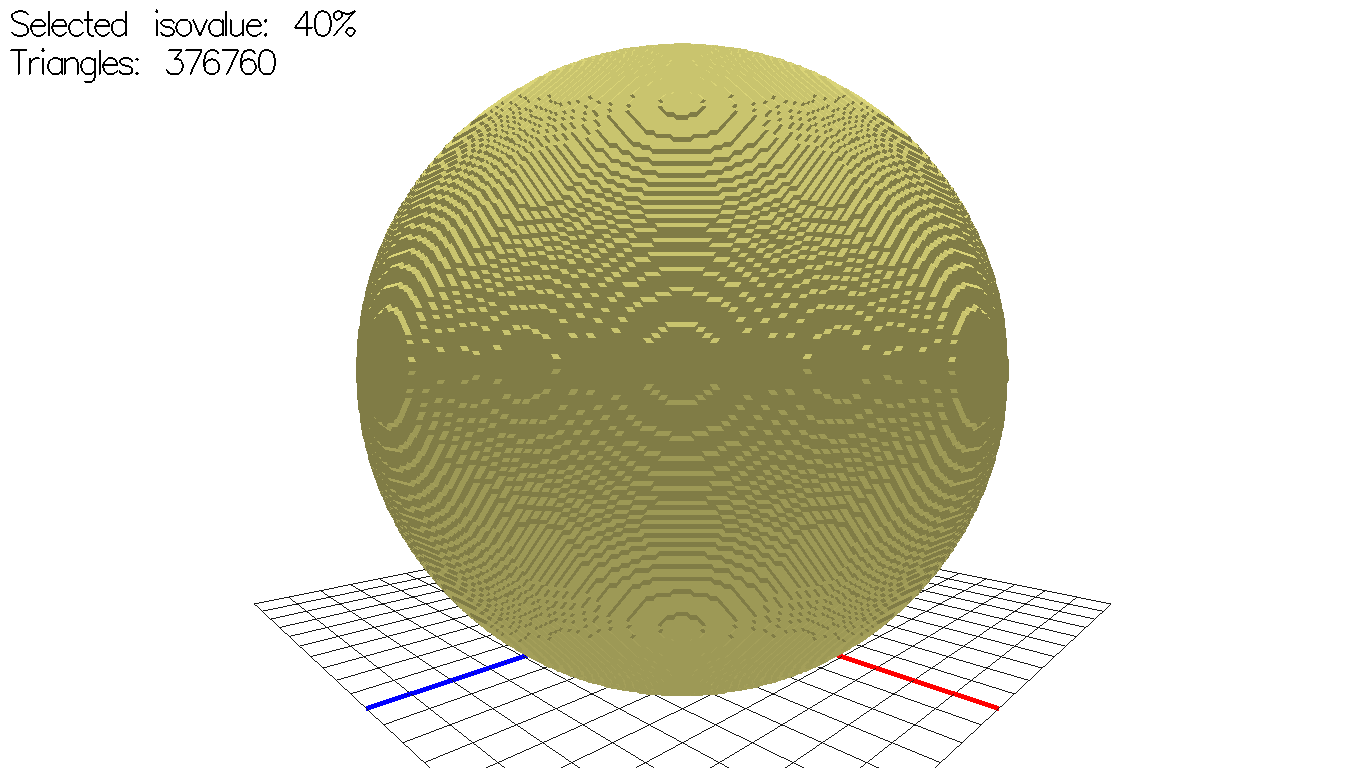
\includegraphics[width=0.95\textwidth]
	{images/results/ImSphRad100/screenshot_40.png}
	\caption{La superficie extraida usando \emph{Marching Cubes} sobre un dataset que describe una esfera.}
	\label{f:implementacion:ImSphRad100:screenshot_40}
\end{figure}

\subsection{Formato de las imágenes de entrada}
\label{ch:implementacion:sec:datosDeEntrada:subsec:formatodelasimagenesdeentrada}

\chapter{Conclusiones}
\label{ch:conclusiones}

Las mallas geométricas son una gran herramienta dentro de la ciencia e ingeniería, sus 
aplicaciones son muchas, y en general se usan para representar un objeto o cuerpo 
discretizadamente.

Por esto, y debido a las implicaciones físicas, es que no se puede hacer un estudio 
infinitesimal de los cuerpos en tres dimensiones y es necesario crear modelos discretizados de 
ellos, para facilitar el trabajo con estos.

Para los fines de visualización, existen diversas técnicas basadas en elementos finitos 
como Marching Squares, Marching Cubes y Marching Tetrahedrons, los cuales, dependiendo de 
su dimensión y objetivos, son capaces de extraer de manera discretizada el contorno o superficie 
de un cuerpo en estudio, para finalmente poder trabajar con él.

No obstante, estos métodos presentan problemas causados por la discretización misma que 
genera malas aproximaciones y para mejorarlas requieren de mayor poder de cómputo, o también 
presentan problemas topológicos causando errores de cálculo importantes. Aún así, hasta la fecha 
se han investigado y aún se pueden crear nuevas técnicas para poder enfrentar estas situaciones, y 
generar mallas cada vez de mayor calidad.


%esto ya esta en Abstract
%\section{Objetivos}
\label{ch:objetivos}

En esta investigación, se estudiarán las distintas técnicas que se han expuesto en el estado del arte, 
se comprobarán los problemas topológicos que traen y se estudiarán las mejoras que actualmente 
se han implementado durante la existencia de estos algoritmos, para que finalmente, se pueda 
proponer un flujo de trabajo que permita, a partir de una nube de puntos, poder extraer una 
superficie del volumen de alta calidad.


%\backmatter
%\cleardoublepage

\singlespacing
\cleardoublepage

\bibliographystyle{plain}
\bibliography{bib/papers}

%\appendix
%\input{include/appendix.tex}

\appendix

%\addcontentsline{toc}{chapter}{Appendix}
%\input{include/Appendix.tex}

\end{document}